\documentclass[aspectratio=169]{beamer}
\usepackage{babel}
\usepackage{array, colortbl, tikz, transparent, listings, pgfplots}
\usepackage[export]{adjustbox}
\usepackage[skins,theorems]{tcolorbox}
\usepackage[dvipsnames]{xcolor}
\usepackage[backend=biber,style=verbose-ibid,citetracker=true,ibidtracker=constrict,autocite=footnote]{biblatex}

\setbeamercovered{transparent}
\lstdefinelanguage{Rust}{
    sensitive=true,
    morekeywords={as, break, const, continue, crate, else, enum, extern, false, fn, for, if, impl, in, let, loop, match, mod, move, mut, pub, ref, return, self, Self, static, struct, super, trait, true, type, unsafe, use, where, while, async, await, dyn, Result, Option, Ok, Err, panic},
    morecomment=[l]{//},
    morecomment=[s]{/*}{*/},
    morestring=[b]",
    morestring=[b]',
}
\lstdefinelanguage{Yaml}{
    sensitive=true,
    morekeywords={true, false, null, particles, type, cuboid, foreach, position, velocity, mass, sigma, brownian_sigma},
    morecomment=[l]{\#},
    morestring=[b]",
}
\lstset{
    language=Rust,
    basicstyle=\ttfamily\small,
    keywordstyle=\color{blue}\bfseries,
    stringstyle=\color{red},
    commentstyle=\color{teal},
    morekeywords={Result, Option, Ok, Err, Some, None, panic},
    breaklines=true
}
\usetikzlibrary{automata,positioning}
\addbibresource{Reference.bib}
\addbibresource{../thesis/literature.bib}

\title{Comparing Molecular Dynamics Simulations with Rust and C++}
\author{Anatoly Weinstein}
\date{16th September 2026}

\newcommand{\framebackground}[3]{
    \begin{tikzpicture}
        \transparent{#1}
        \node[inner sep=0] at (current page.center) {
            
\includegraphics[height=\paperheight, right]{media/tum-uhrenturm.png}
        };
        \transparent{#2}
        \node[anchor=south, text width=\paperwidth, text height=1.5cm, draw=none, align=center] at (current page.south) {
            \insertpagenumber
        };
        \transparent{#3}
        \node[anchor=south, text width=\paperwidth, text height=1.5cm, draw=none, align=right] at (current page.south) {
            \small Anatoly W. \,\,
        };
    \end{tikzpicture}
}

\newcommand{\headerframe}{
    \usebackgroundtemplate{
        \framebackground{0.2}{1}{1}
    }
}

\newcommand{\simpleframe}{
    \usebackgroundtemplate{
        \framebackground{0}{1}{1}
    }
}

\newcommand{\nofooterframe}{
    \usebackgroundtemplate{
        \framebackground{0}{0}{1}
    }
}

\newcommand{\blue}[1]{{\color{beamer@blendedblue} #1}}
\newcommand{\yellow}[1]{{\color[HTML]{AF8F10} #1}}
\newcommand{\gray}[1]{{\color[HTML]{8F8F8F} #1}}
\newcommand{\red}[1]{{\color[HTML]{FF5F5F} #1}}

\begin{document}

%
% Frame
%
\usebackgroundtemplate{\framebackground{0.2}{0}{0}}
\begin{frame}
    \maketitle
\end{frame}

\simpleframe\begin{frame}{Table of Contents}
    \tableofcontents
\end{frame}

\section{Motivation and Background}
\simpleframe\begin{frame}[t]{Motivation and Background}
    \begin{figure}
        \centering
        \includegraphics[width=0.8\textwidth]{media/hello-particles.png}
    \end{figure}

    Simulating particle physics is expensive: The pair interaction problem for force calculation is in $\mathcal O(n^2)$. Other than algorithmic optimizations, choice of language can have an impact on performance.
\end{frame}

\nofooterframe\begin{frame}[t]{Motivation and Background}
    \begin{figure}[h!]
    \begin{tikzpicture}
        \begin{axis}[
            width=0.7\textwidth,  
            height=0.6\textheight,
            xlabel={Year},
            % ylabel={Percentage},
            ylabel={Percentage Admired},
            xtick={2010, 2015, 2020, 2025},
            scaled x ticks=false,  
            scaled y ticks=false,
            ymajorgrids=true, 
            grid style=dashed,
            ymin=-5,
            ymax=105,
            xmin=2014,
            xmax=2026,
            x tick label style={/pgf/number format/.cd, 1000 sep={}},
            % legend style={at={(0.02,0.45)},anchor=north west},
            legend style={at={(0.07,0.35)},anchor=north west},
        ]

        \addplot[
            color=blue,
            mark=square,
            line width=1pt,
            ]
            coordinates {
                (2015, 75.6)(2017, 52.0)(2018, 46.7)(2019, 52.0)(2020, 43.4)(2021, 49.2)(2022, 48.4)(2023, 49.8)(2024, 53.1)(2025, 46.6)
            };

        \addplot[
            color=Bittersweet,
            mark=triangle,
            line width=1pt,
            ]
            coordinates {
                (2015, 73.8)(2016, 79.1)(2017, 73.1)(2018, 78.9)(2019, 83.5)(2020, 86.1)(2021, 86.9)(2022, 86.7)(2023, 84.7)(2024, 82.2)(2025, 72.4)
            };

        % \addplot[
        %     color=cyan,
        %     mark=square,
        %     line width=1pt,
        %     ]
        %     coordinates {
        %         (2023, 16.4)(2024, 18.3)(2025, 16.7)
        %     };

        % \addplot[
        %     color=Dandelion,
        %     mark=triangle,
        %     line width=1pt,
        %     ]
        %     coordinates {
        %         (2023, 30.6)(2024, 28.7)(2025, 29.9)
        %     };

        \legend{C++, Rust}
        % \legend{C++ (Admired), Rust (Admired), C++ (Desired), Rust (Desired)}
        \end{axis}
    \end{tikzpicture}
    \end{figure}

    In recent years, Rust has gained a lot of popularity and reputation as a strong C++ contender in memory-safety and performance. It was also rated ``the most admired programming language'' in the StackOverflow developer surveys\footcite{stackoverflow-developer-survey}.
\end{frame}

\section{The Rust Programming Language}
\headerframe\begin{frame}{}
    \centering
    \Large
    \blue{The Rust Progrogramming Language}
\end{frame}

\subsection{The Cargo Ecosystem}
\simpleframe\begin{frame}{The Cargo Ecosystem}
    \begin{tabular}{ m{0.46\textwidth} | m{0.46\textwidth} } 
        \textbf{Rust} & \textbf{C++} \\
        \hline
        \texttt{cargo build} & \texttt{make} \\
        \texttt{cargo run} & \texttt{make \&\& ./out.o} \\
        \texttt{cargo test} & \texttt{ctest} \\
        \texttt{cargo doc} & \texttt{doxygen} \\
        \texttt{cargo fmt} & \texttt{clang-format} \\
        \texttt{cargo clippy} & \texttt{clang-tidy} \\
    \end{tabular}

    \vspace{1.5em}
    Rust is installed with its package manager \blue{Cargo}, which manages the toolchain for Rust as subcommands.
    % It comes with the tester, formatter and linter, and other subcommands.
    The C++ ecosystem is more fragmented, adding dependencies is done manually with CMake, so is the configuration of testing and documentation generators.
\end{frame}

\subsection{The Ownership Model}
\simpleframe\begin{frame}[t]{The Ownership Model}{Ownership}
    Rust guarantees memory safety and automatically frees memory when a value goes out of scope. This is achieved through the ``Ownership model'', a set of rules which are enforced at compile time.

    {\centering
    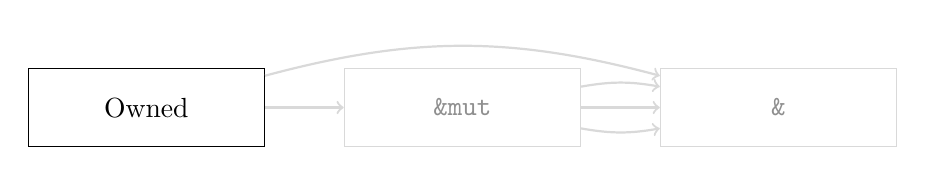
\begin{tikzpicture}[node distance=1cm and 1cm, minimum height=1cm, minimum width=3cm]
        \node[draw, rectangle] (owned) {Owned};
        \node[draw, rectangle, gray!30, right=of owned] (mutborrow) {\gray{\texttt{\&mut}}};
        \node[draw, rectangle, gray!30, right=of mutborrow] (borrow) {\gray{\texttt{\&}}};

        \draw[->, gray!30, thick] (owned) -- (mutborrow) node[midway, above] {};
        \draw[->, gray!30, thick] (mutborrow) -- (borrow) node[midway, above] {};
        \draw[->, gray!30, thick] (mutborrow) to[bend left = 10] (borrow) node[midway, above] {};
        \draw[->, gray!30, thick] (mutborrow) to[bend right = 10] (borrow) node[midway, above] {};
        \draw[->, gray!30, thick] (owned) to[bend left = 15] (borrow) node[midway, above] {};
    \end{tikzpicture}
    \vspace{1em}

    \begin{description}
        \item[\blue{Rule 1}] The value has an owner,
        \item[\blue{Rule 2}] and only one owner at any time.
        \item[\blue{Rule 3}]  When the owner leaves the scope, without passing on ownership, the value will be dropped.
    \end{description}}

    \blue{Intuition:} The scope of the owner defines the \blue{lifetime} of a value.
\end{frame}

\simpleframe\begin{frame}[t,fragile]{The Ownership Model}{Ownership}
    \begin{lstlisting}[frame=single,breaklines=false]
fn problematic_move() {
    let s = String::from("hello");
    {                // inner scope
        let t = s;   // a is moved to b
    }                // b goes out of scope
    println!("{s}"); // error: use of moved value
}
    \end{lstlisting}
    \vspace{0.5em}

    This example breaks \blue{Rule 2: There can only be one owner}. When \texttt{b} goes out of scope, the value is freed.
\end{frame}

\simpleframe\begin{frame}[t]{The Ownership Model}{Borrowing and References}
    To make sure values can be shared across different scopes, Rust introduces the concept of \blue{borrowing}: When references go out of scope, the value is not dropped, and a reference cannot outlive its value.

    {\centering
    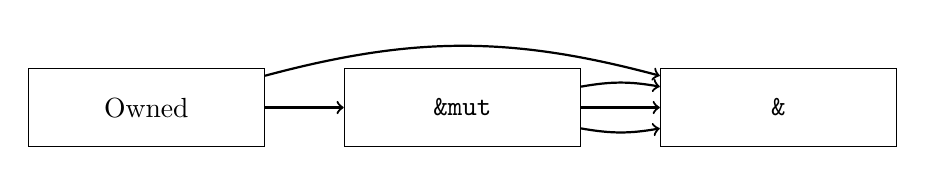
\begin{tikzpicture}[node distance=1cm and 1cm, minimum height=1cm, minimum width=3cm]
        \node[draw, rectangle] (owned) {Owned};
        \node[draw, rectangle, right=of owned] (mutborrow) {\texttt{\&mut}};
        \node[draw, rectangle, right=of mutborrow] (borrow) {\texttt{\&}};

        \draw[->, thick] (owned) -- (mutborrow) node[midway, above] {};
        \draw[->, thick] (mutborrow) -- (borrow) node[midway, above] {};
        \draw[->, thick] (mutborrow) to[bend left = 10] (borrow) node[midway, above] {};
        \draw[->, thick] (mutborrow) to[bend right = 10] (borrow) node[midway, above] {};
        \draw[->, thick] (owned) to[bend left = 15] (borrow) node[midway, above] {};
    \end{tikzpicture}
    \vspace{1em}

    \begin{description}
        \item[\blue{Rule 4}] At any given time, an item can either have one mutable reference or multiple immutable references,
        \item[\blue{Rule 5}] and any reference must be valid (no dangling references!).
    \end{description}}

    \vspace{1.5em}
    \blue{Intuition:} Owner can read, write and free. Mutable borrow can read and write. Immutable borrow can only read.
\end{frame}

\simpleframe\begin{frame}[t,fragile]{The Ownership Model}{Borrowing and References}
    \begin{lstlisting}[frame=single,breaklines=false]
fn too_many_references() {
    let s = String::from("hello");
    let muts = &mut s; // 'muts' is a mutable borrow of 's'
    println!("{s}");   // problem: printing a value borrows it
                       // immutable (reading value content)
                       // 'muts' out of scope
}
    \end{lstlisting}
    \vspace{0.5em}

    This example breaks \blue{Rule 4: Either one mutable reference or multiple immutable}.
\end{frame}

\simpleframe\begin{frame}[t,fragile]{The Ownership Model}{Borrowing and References}
    \begin{lstlisting}[frame=single,breaklines=false]
fn dangle() -> &String {
    let s = String::from("hello");
    return &s; // returns a reference to s;
               // s goes out of scope => &s is invalid
}
    \end{lstlisting}
    \vspace{0.5em}

    This example breaks \blue{Rule 5: Any reference must be valid}. 
    % Dangling references are a common problem in Rust when writing function chains:

%     \begin{lstlisting}[frame=single,breaklines=false]
% vec!["Hello", "World", "Banana"] // type equivalent: std::vector<std::string>
%     .iter()
%     .map(|value| &String::from(value)) // not allowed
%     \end{lstlisting}
\end{frame}

\subsection{Traits vs Interfaces}
\simpleframe\begin{frame}{Traits vs Interfaces}
    trait
\end{frame}

\subsection{Dynamic Dispatch}
\simpleframe\begin{frame}{Dynamic Dispatch}
    dyn
\end{frame}

\section{Implementation}
\headerframe\begin{frame}{}
    \centering
    \Large
    \blue{Implementation}
\end{frame}

\subsection{Direct Sum}
\simpleframe\begin{frame}{Direct Sum}
    sum
\end{frame}

\subsection{Linked Cells}
\simpleframe\begin{frame}{Linked Cells}
    cells
\end{frame}

\subsection{Parallel}
\simpleframe\begin{frame}{Parallel}
    par
\end{frame}

\section{Benchmarks}
\headerframe\begin{frame}{}
    \centering
    \Large
    \blue{Benchmarks}
\end{frame}

\simpleframe\begin{frame}{Mars}
    \begin{figure}
        \centering
        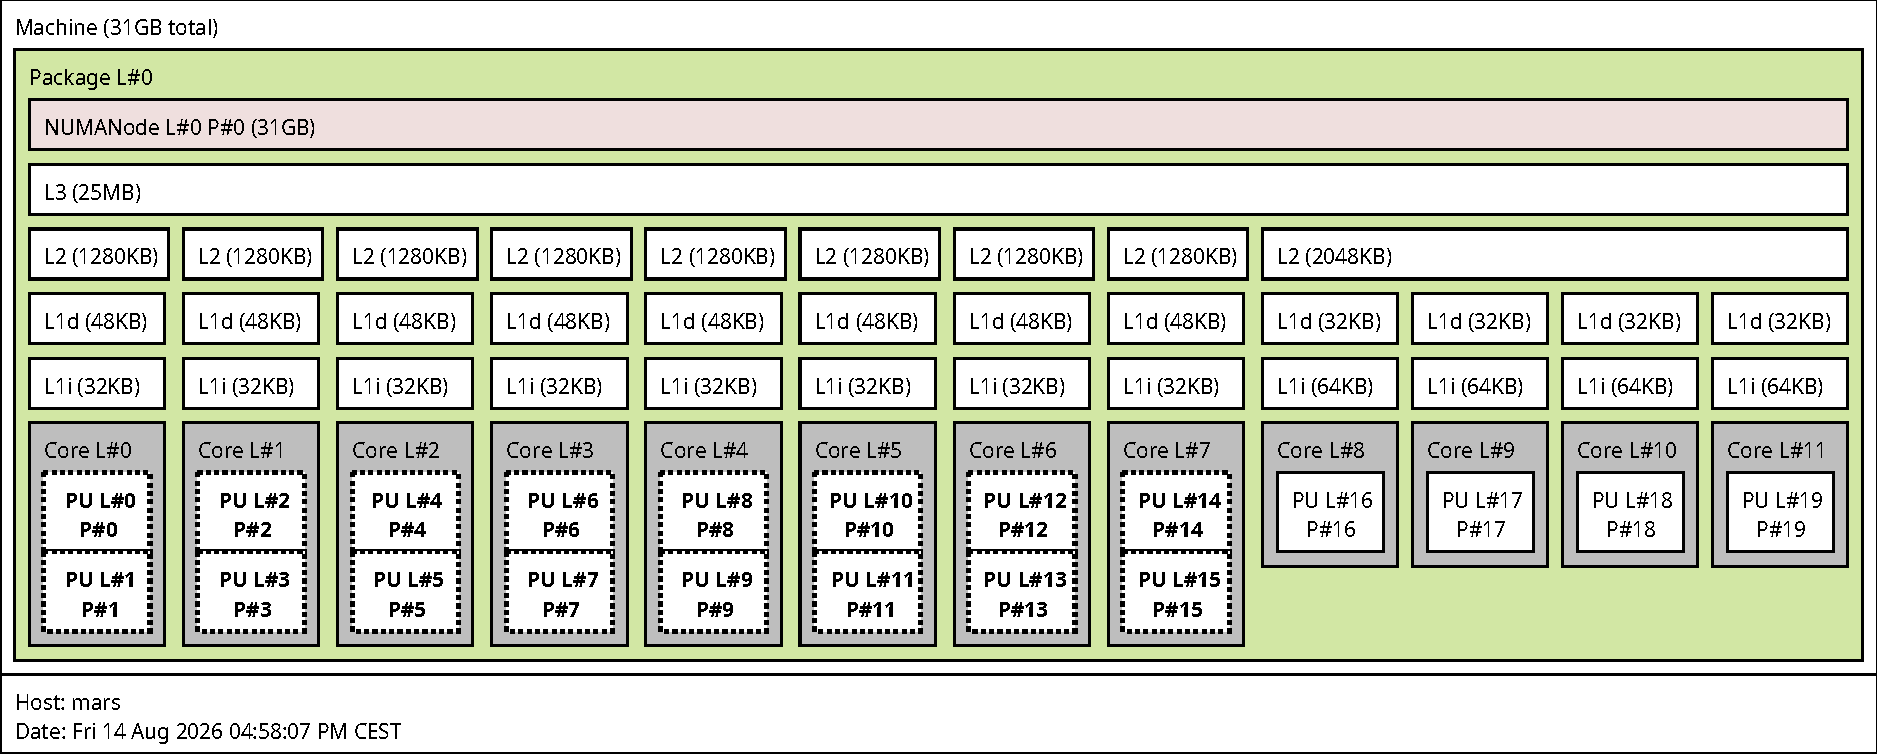
\includegraphics[width=0.8\textwidth]{../hwloc_diagram.pdf}
    \end{figure}

    The benchmarks were run on my high-end PC ``mars'' and the CoolMUC supercluster. Mars runs on a \blue{64-bit 12th Gen Intel(R) Core(TM) i7-12700K} which has \blue{8 performance cores with a pair of threads} and \blue{4 efficiency cores}, accounting for \blue{20 hardware threads}\footnote{$8 \cdot 2 + 4 \cdot 1 = 20$}.
\end{frame}

\headerframe\begin{frame}[allowframebreaks]{References}
  \printbibliography
\end{frame}

\section{Appendix}
\headerframe\begin{frame}{}
    \centering
    \Large
    \blue{Appendix}
\end{frame}

\simpleframe\begin{frame}{Ownership and Borrowing: Rules}
    \begin{enumerate}
        \item The value has an owner,
        \item and only one owner at any time.
        \item  When the owner leaves the scope, without passing on ownership, the value will be dropped.
        \item At any given time, an item can either have one mutable reference or multiple immutable references,
        \item and any reference must be valid (no dangling references!).
    \end{enumerate}
\end{frame}

\end{document}
